\documentclass{article}
\usepackage[margin=3cm]{geometry}
\usepackage[utf8]{inputenc}
\usepackage{amsmath}
\usepackage{amssymb}
\usepackage{float}
\usepackage{enumitem}
\usepackage{graphicx}
\usepackage{caption}
\usepackage{subcaption}

\graphicspath{ {plots/} }

\title{Nonlinear Optimization - Homework 1 }
\author{Christian Segercrantz 481056}


\begin{document}
	\maketitle
	\pagebreak
\section*{2.1}
\begin{equation} \label{eq:1}
	f(x) = x_1^3-x_1+x_2^3-x_2
\end{equation}
\subsection*{(a)}
	\begin{figure}[H]
		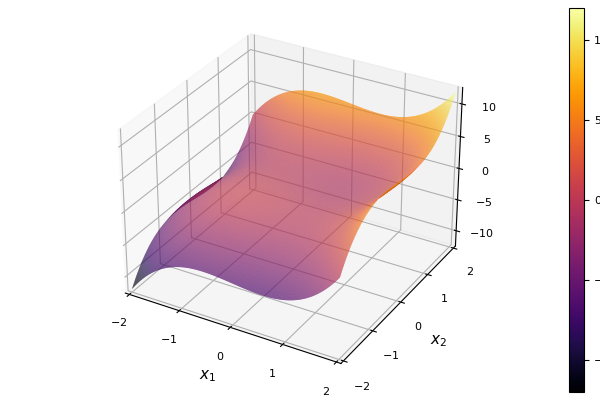
\includegraphics[width=0.8\textwidth]{H21_surface.png}
		\caption{The surface plot of equation \eqref{eq:1}.}
		\label{fig:1a}
	\end{figure}
	By examining Figure \ref{fig:1a}, I would conclude that the function is non-convex as we can clearly see areas that do not follow the definition of a convex function $f(\lambda x_1 + (1 - \lambda)x_2 ) \leq \lambda f(x_1 ) + (1 - \lambda)f(x_2)$.
\subsection*{(b)}
	In order for us to find the critical point, we will solve the first-order derivative of the function.
	\begin{equation}
		\nabla f(x_1,x_2) =
		\begin{bmatrix}
			3x_1^2-1 \\
			3x_2^2-1
		\end{bmatrix}.
	\end{equation}
	The first-order necessary condition is $\nabla f(\bar{x}) = 0$ for our unconstrained problem . We can solve the equations to get the critical points:
	\begin{equation}
		2x^2-1 = 0 \iff x= \pm\sqrt{1/3}.
	\end{equation}
	This gives us the four points $(\sqrt{1/3},\sqrt{1/3})$, $(-\sqrt{1/3},\sqrt{1/3})$, $(\sqrt{1/3},-\sqrt{1/3})$, and $(-\sqrt{1/3},-\sqrt{1/3})$.

\section*{2.2}
	\begin{equation}
		f(x_1,x_2) = 2x^2_1 -x_1x_2+x_2^2 -3x_1 + e^{2x_1+x_2}
	\end{equation}
\subsection*{(a)}
	By corollary 6 of lecture 4, we know that the first-order necessary condition for unconstrained problems is that \textit{"Suppose $f : \mathbb{R}^n \rightarrow \mathbb{R}$ is differentiable at $\bar{x}$. If $\bar{x}$ is a local minimum, then $\nabla f(\bar{x}) = 0$".}	The equation to be satisfied is thus $\nabla f(\bar{x}) = 0$. We calculate $\nabla f$:
	\begin{equation}
		\nabla f =
			\begin{bmatrix}
			4x_1-x_2-3+ 2 e^{2 x_1 + x_2} \\
			-x_1+2x_2 + e^{2x_1+x_2}
			\end{bmatrix}
	\end{equation}
	For this to be a sufficient condition for optimality the function $f(x_1,x_2)$ has to be convex. Then, based on theorem 8 from lecture 4 can we have sufficient conditions. Since we know the following things:
	\begin{enumerate}
		\item Polynomials are convex,
		\item The linear combination of convex functions are convex,
	\end{enumerate}
	we can conclude that the function $f(x_1,x_2)$ is convex. We thus have the necessary and sufficient condition for optimality.
\subsection*{(b)}
	If $\bar{x}=(0,0)$ is to be a optimal point, must it satisfy $\nabla f(0,0) = \boldsymbol{0}$. 
	\begin{align}
		\nabla f =&
			\begin{bmatrix}
				4x_1-x_2-3+ 2 e^{2 x_1 + x_2} \\
				-x_1+2x_2 + e^{2x_1+x_2}
			\end{bmatrix} \\
		=& \begin{bmatrix}
				0-0-3+ 2 e^{0} \\
				-0+0 + e^{0}
			\end{bmatrix}\\
		=& \begin{bmatrix}
				-1 \\
				1
		\end{bmatrix} \neq
		\begin{bmatrix}
			0 \\
			0
		\end{bmatrix}
	\end{align}
	We can see that the point $(0,0)$ does not satisfy the condition.
	
	The direction $d$ that makes the function decrease must satisfy the condition $\nabla f(\bar{x})^\top d <0$.
\subsection*{(c)}
	To find the minimum for $f(x)$ in the direction d= $\begin{bmatrix}-1 \\ 1\end{bmatrix}$ we must calculate the step size $\bar{\lambda}=\text{argmin}_{\lambda} d^\top \nabla(x+ \lambda d)$. We can 
\end{document}